\scanpage{84}
% manuscript line 1
\figure{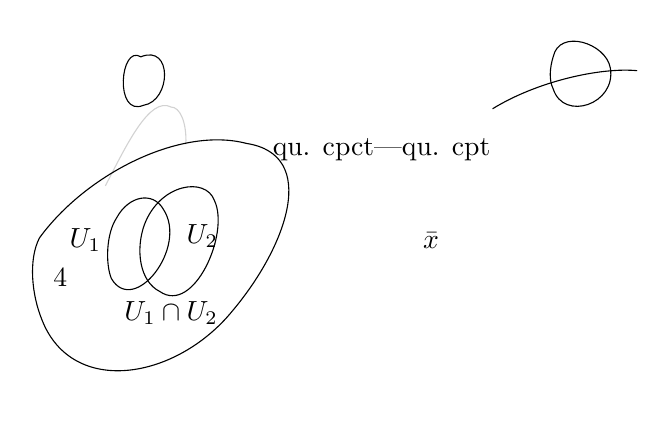
\begin{tikzpicture}[x=.011cm,y=-.011cm]
\draw (42,32) .. controls (18,17) and (11,102) .. (45,88)
 .. controls (77,83) and (79,17) .. (42,32);
\draw[gray!35] (1,181) .. controls (25,135) and (52,77) .. (77,90)
 .. controls (87,90) and (95,107) .. (94,133);
\draw (-75,241) .. controls (-21,167) and (88,112) .. (164,132)
 .. controls (248,145) and (211,250) .. (148,325)
 .. controls (83,405) and (-37,425) .. (-72,336)
 .. controls (-84,307) and (-88,266) .. (-75,241);
\draw (14,218) .. controls (28,192) and (56,187) .. (68,208)
 .. controls (97,252) and (34,332) .. (8,288)
 .. controls (1,271) and (2,236) .. (14,218);
\draw (46,226) .. controls (64,178) and (117,170) .. (127,198)
 .. controls (145,236) and (103,330) .. (64,303)
 .. controls (40,291) and (36,254) .. (46,226);
\node at (-22,244) {$U_1$}; \node at (113,239) {$U_2$};
\node at (77,328) {$U_1\cap U_2$}; \node at (-51,287) {$4$};
\node[anchor=west] at (183,139) {\unsure{qu. cpct|qu. cpt}};
\draw (518,32) .. controls (525,-1) and (579,16) .. (584,45)
 .. controls (591,87) and (530,107) .. (518,69) .. controls (513,59) and (514,45) .. (518,32);
\draw (448,92) .. controls (500,60) and (573,44) .. (615,48);
\node at (377,244) {$\bar x$};
\end{tikzpicture}}

% manuscript line 2
\margin{Supposons que tt pt de $X$ a un syst. fond. de voisinages ouverts, rétrocompacts dans $X$. [Alors tte partie ouverte quasi-cpte de $X$ est rétrocompacte]}
\par\noindent\rule{.94\linewidth}{.3pt}

% manuscript line 5
\margin{$\unsure{E|F|Z}$\par $U$}
Soit $\deleted{\unsure{F|E}}T$ une partie fermée irréductible de $X$.

% manuscript line 6
Conditions équivalentes

% manuscript line 7
(i) Il existe une partie $Z$, ouverte non vide dans $T$, telle que $Z$ soit constructible \unsure{dans} $X$

% manuscript line 9
(ii) Il existe un ouvert \inserted{quasi-compact} $U$ de $X$, tel que $U\cap T\ne\varnothing$, et $U-U\cap T$ soit quasi cpct.
% archive sheet number: 83
% Faint type visible in reverse is on the other face of the paper.
